\subsection{Máquina Virtual de Nebulas (\textit{Nebulas Virtual Machine}, NVM)}
\label{sec:nvm}

LLVM \cite{llvm} es el componente central de la NVM, y el bytecode LLVM se utiliza como bytecode NVM.

El bytecode de la NVM se compila de forma dinámica, se optimiza por medio del JIT LLVM y se ejecuta en el entorno \textit{sandbox} de NVM. Gracias a esta arquitectura, la performance y la seguridad del código del núcleo y de los contratos inteligentes en Nebulas se puede mejorar continuamente mediante LLVM.

LLVM es una colección de \textit{toolchains} y tecnologías de compilación altamente modulares, que se utilizó previamente como \textit{framework} de compilación de código en Google, Apple y muchas otras empresas. LLVM proporciona representaciones intermedias neutrales (LLVM IR) y una infraestructura de compilación acorde, y ofrece un nuevo conjunto de estrategias de compilación con respecto a esta infraestructura, incluyendo la optimización de LLVM IR, la generación de código de LLVM IR a bytecode LLVM y la ejecución directa del bytecode LLVM en diferentes plataformas de hardware a través del JIT LLVM, tal como se muestra en la \reffig{fig:llvm}. \\

\begin{figure}[h]
\centering
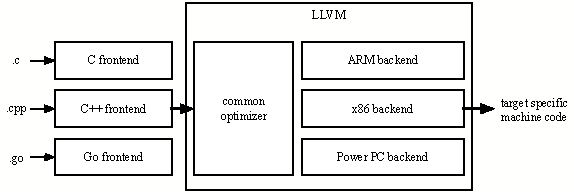
\includegraphics[width=10cm]{./figs/llvm}
\caption{LLVM}
\label{fig:llvm}
\end{figure}

Desarrollamos la NVM basándonos en LLVM (véase \reffig{fig:nvm}). En primer lugar, proporcionamos las librerías API subyacentes para blockchain. Luego, creamos un \textit{frontend} para el compilador, disponible en diferentes lenguajes tales como Solidity, JavaScript, C, C++, Go, etc. A continuación, utilizamos el \textit{toolchain} proporcionado por LLVM para generar el bytecode LLVM. Finalmente, este bytecode LLVM se ejecuta en un \textit{sandbox} proporcionado por NVM a través del motor JIT de LLVM.

\begin{figure}[h]
\centering
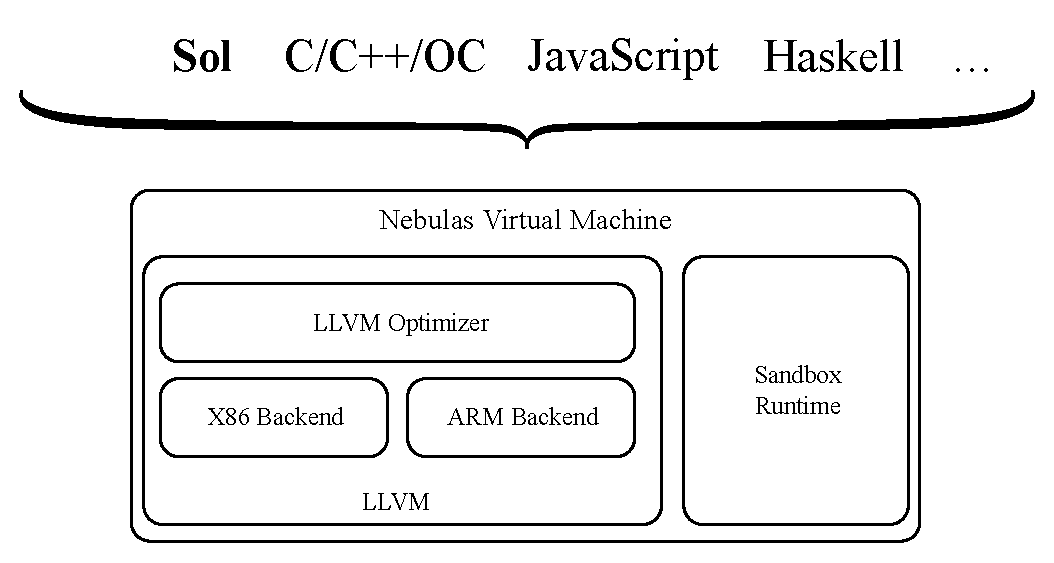
\includegraphics[width=10cm]{./figs/nvm}
\caption{Máquina Virtual de Nebulas}
\label{fig:nvm}
\end{figure}

La Máquina Virtual de Nebulas es la piedra angular de Nebulas Force. Cuando se libera un nuevo código de protocolo o un contrato inteligente, el bytecode LLVM se genera luego de que el nuevo código es compilado por LLVM en NVM, y es liberado al blockchain. Una vez confirmado allí, el nuevo código será compilado y optimizado por LLVM JIT, y colocado en el sandbox para reemplazar el código viejo y ser ejecutado, tal como se muestra en la \reffig{fig:nvm-process}.

\begin{figure}[h]
\centering
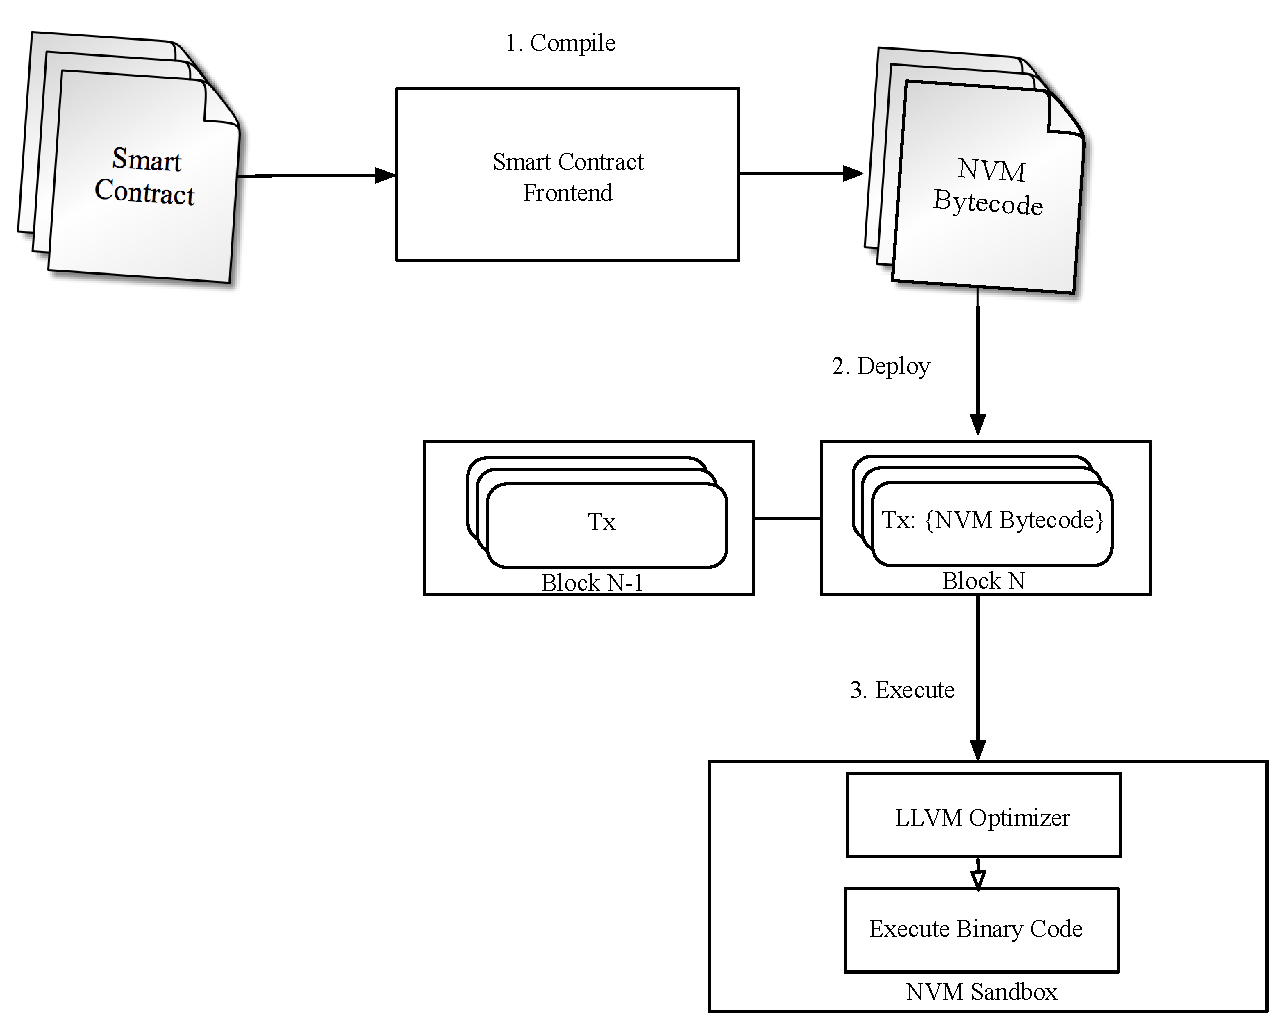
\includegraphics[width=10cm]{./figs/nvm-process}
\caption{El mecanismo de operación de la Máquina Virtual de Nebulas}
\label{fig:nvm-process}
\end{figure}

Con LLVM (véase \reffig{fig:llvm}), NVM también ayuda a los desarrolladores a escribir contratos y aplicaciones inteligentes por medio de sus lenguajes de programación favoritos, como Solidity, JavaScript, e incluso Haskell. Además de estos populares lenguajes, NVM también da soporte a lenguajes personalizados de alto nivel para diferentes áreas y escenarios, tales como DSL para sistemas financieros. Estos lenguajes de alto nivel son más fáciles de verificar formalmente, mejorando aún más la robustez y seguridad del código, algo que permite a los desarrolladores escribir contratos y aplicaciones más sofisticadas.